\chapter{RESULTS AND DISCUSSION}
In this chapter we are going to present various result that we have got from our implementation 
\section{TWEETS COLLECTED}
We collected tweets  by using Twitter API.  A .json file is generated each time when we ran our Python script for tweets fetching. This file consists of original text message of tweets as well as many other information. We removed all other unnecessary information and created a data set which consists only original text.
A sample file of tweets is shown in Figure:
\begin{figure}[h]
\label{sct}
\centerline{\includegraphics[width=4in]{sct}}
\caption{Sample cleaned tweets}
\end{figure}
We collected 26,239  tweets between  30th July 2017 and  6th August 2017.
Number of tweets collected per day is shown in Figure :

\begin{figure}[h]
\label{ut}
\centerline{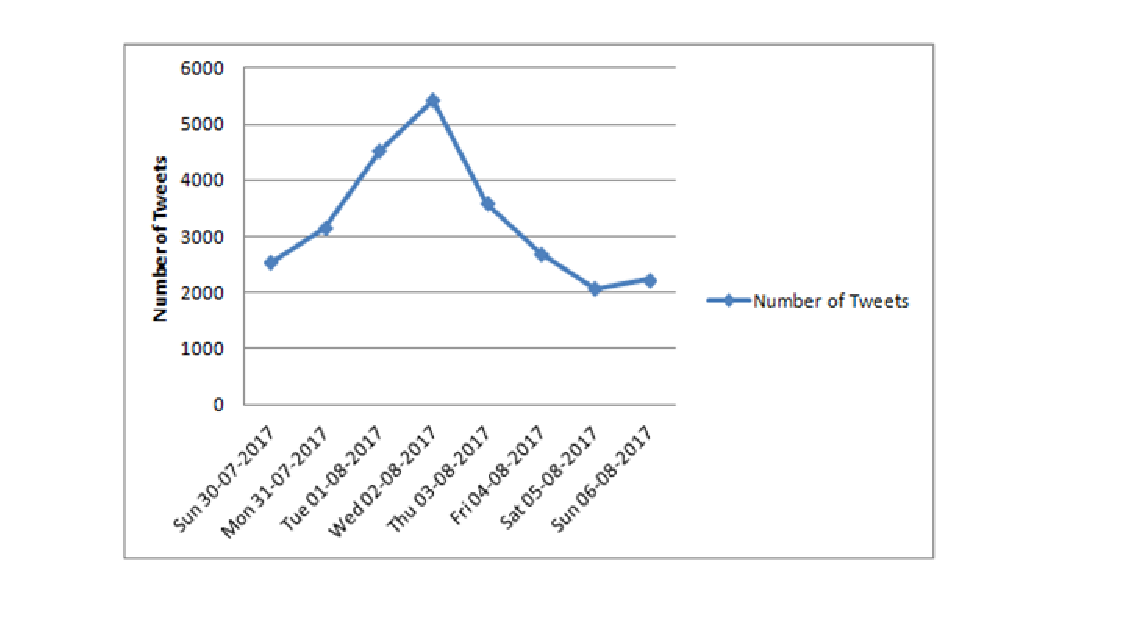
\includegraphics[width=4in]{ut}}
\caption{Collected tweets per day}
\end{figure}
\section{TWITTER  DATA ANALYSIS }
For our thesis , we collect tweets which consists keywords 'Zika'  continuously  for eight days .We pre-process our dataset so that we can use them for sentiment classification. We are going to pass our dataset to the Naive Bayes  classifier .Sample tweets with its polarity are  shown in Figure:
 \begin{figure}[h]
\label{ftw}
\centerline{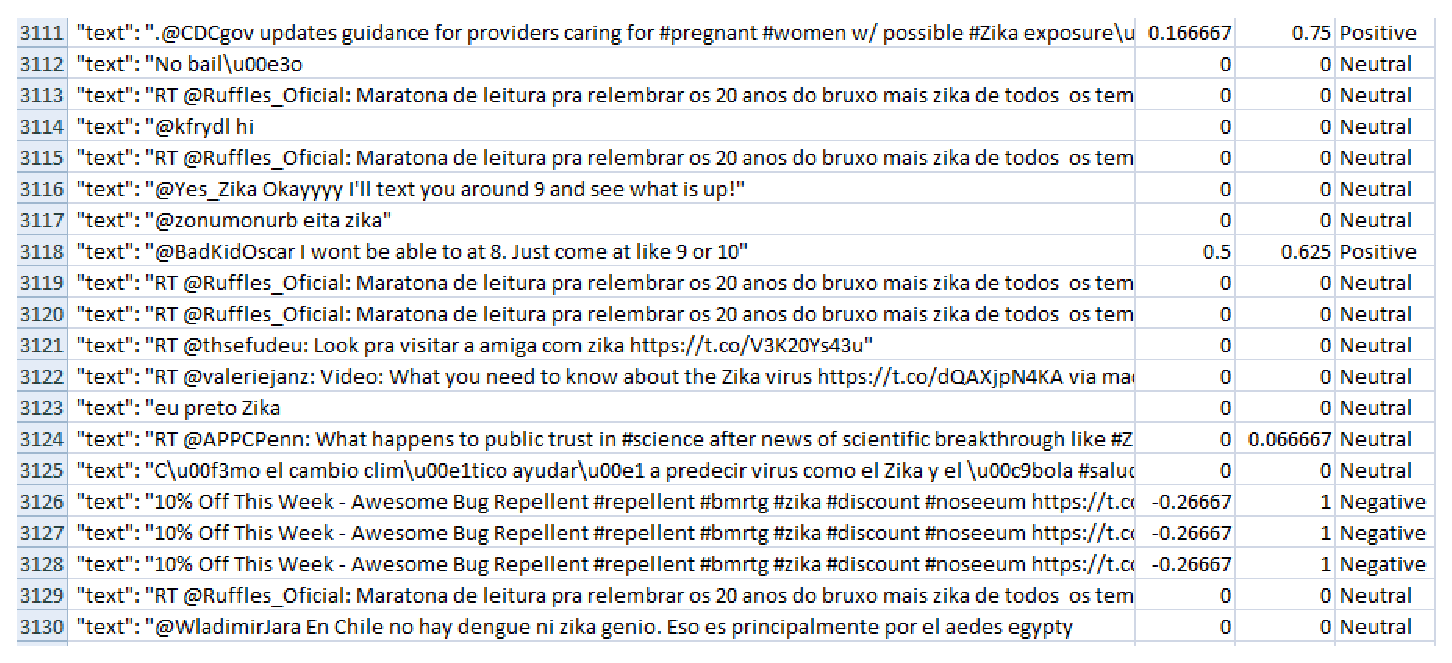
\includegraphics[width=4in]{ftw}}
\caption{Filtered tweets with output}
\end{figure}
When we ran our Python script for sentiment polarity on dataset which consists of 26239 , it classifies data into their  polarity and printed out result in terms of numbers as well as percentage. In IPython console it  printed the result which is shown in Figure:  
 \begin{figure}[h]
\label{ut1}
\centerline{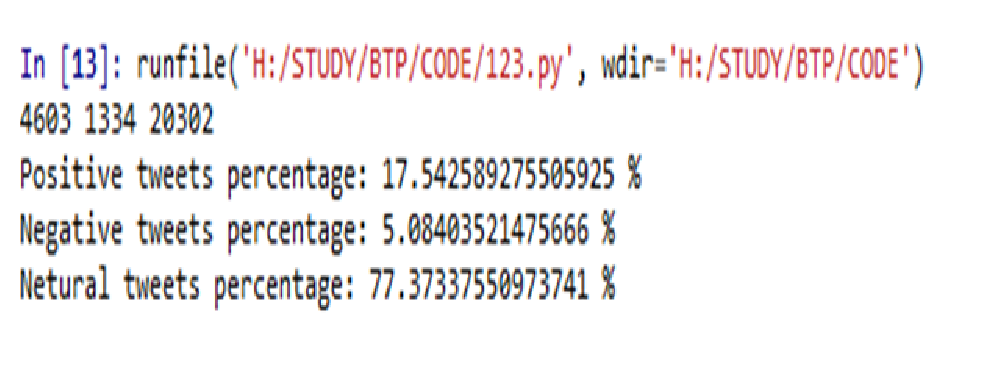
\includegraphics[width=4in]{ut1}}
\caption{In Python console printed the result }
\end{figure}
The Python script classified 20302 tweets as neutral , 4603 as positive and 1334  as negative . 
\begin{table}
 \begin{tabular}{|c c c|}
 \hline
 Polarity & Number of tweets & Percentage of tweets(\%) \\ 
 \hline
 Positive & 4603 & 17.54 \\
 \hline
 Negative & 1334 & 5.08 \\
 \hline
 Neutral & 20302 & 77.37 \\ 
 \hline
\end{tabular}
\end{table}
 \begin{figure}[h]
\label{ut2}
\centerline{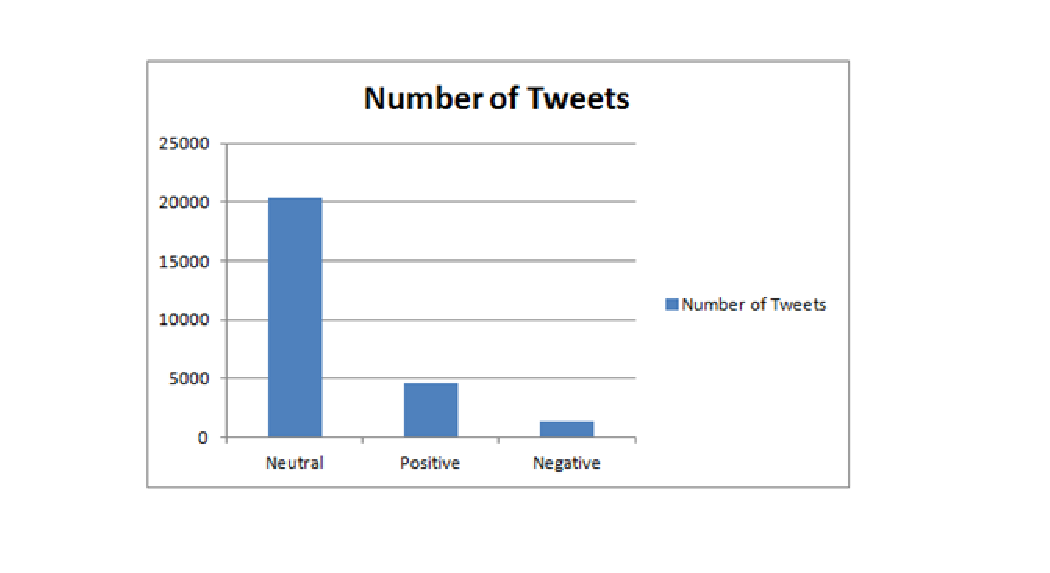
\includegraphics[width=4in]{ut2}}
\caption{Graph between polarity and number of tweets}
\end{figure}
In a similar study done in 2016 \cite{edtr10} they found  that as much as 59 \% of the tweets on Zika virus was negative, and that was the time when WHO (World Health Organization) declared emergency \cite{edtr11,edtr12} because there were estimated  millions of cases from around the world was reported during 2015 - 2016. Therefore there was very high level of concern among society  regarding this epidemic  and hence it was clearly visible in the report where 59 \%  of tweets were negative . In our study we  found that only  5.08 \%  tweets are negative. Because we have done  our study at  such a time when Zika virus is no longer a matter of high concern among people.
\par So by  comparing these two results it is clear that Twitter could play a major role in case of any epidemic or public health emergency to decide the level of concern among people by using sentiment analysis.
 \begin{figure}[h]
\label{ut3}
\centerline{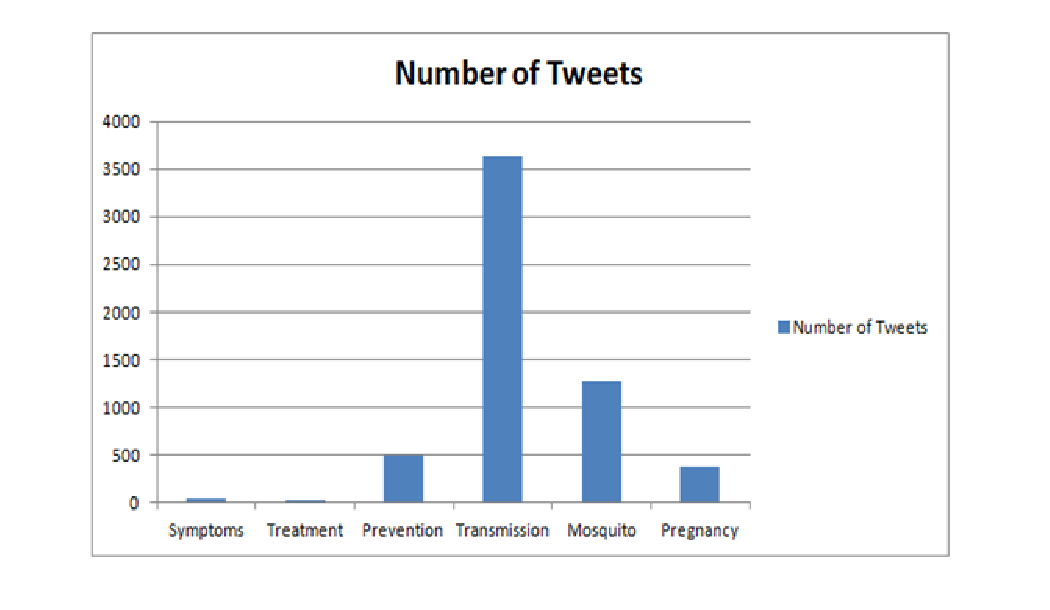
\includegraphics[width=4in]{ut3}}
\caption{Number of tweets in each categorization after running all tweets}
\end{figure}
We have analyzed all the tweets by dividing  them in six categories which are Symptoms, Treatment, Prevention , Transmission, Mosquito and Pregnancy. We included two other classes along with four diseases characteristics. Since Zika virus is spread through  mosquitoes and a pregnant mother could pass the Zika virus to her infant  . These are the two main reasons we included two other classes Mosquito and Pregnancy .
We found that very high number of people were tweeting  about the four diseases characteristics , mosquito and pregnancy which shows that very large number of people were tweeting relevant to this epidemic.
\par After analyzing the data we found that most number of people were twitting about transmission , mosquito and prevention . Not many people were twitting about treatment , the reason for that is there is not any convincing  treatment for Zika virus  . Sample tweets from all these categories are shown in table :

